\documentclass[a4paper,USenglish,cleveref, autoref]{lipics-v2021}
\usepackage[utf8]{inputenc}
\usepackage{xspace}
\usepackage{listings}
\usepackage{wrapfig}
\usepackage{multicol}
\usepackage{comment}
\usepackage{tikz}
\usepackage{xspace}

% \usepackage[frozencache]{minted}
\usepackage{minted}

%\usemintedstyle{ssr}
\usemintedstyle{tango}
\setminted{fontsize=\small,frame=single}
 

%\excludecomment{minted} \renewcommand{\inputminted}{CODE: } % compile without code

\begin{comment}
\begin{figure}
  \begin{multicols}{2}
    \inputminted{snippets/change.v}
  \end{multicols}
  \caption{\MK{CHANGEME}}
  \label{fig:copy}
\end{figure}
\end{comment}

\DeclareUnicodeCharacter{2200}{$\forall$}
\DeclareUnicodeCharacter{2218}{$\circ$}
\DeclareUnicodeCharacter{2080}{$_0$}
\DeclareUnicodeCharacter{2081}{$_1$}
\DeclareUnicodeCharacter{2082}{$_2$}
\DeclareUnicodeCharacter{03BB}{$\lambda$}
\DeclareUnicodeCharacter{2248}{$\approx$}

\newcommand{\M}[1]{\mintinline{coq}{#1}}
%\newcommand{\M}[1]{M}
\newcommand{\Adv}{\mathrm{Adv}}
\newcommand{\A}{\mathcal{A}}
\renewcommand{\P}{\mathcal{P}}
\newcommand{\CPA}{\ensuremath{\mathrm{PK\text{-}CPA}}}
\newcommand{\OTS}{\ensuremath{\mathrm{PK\text{-}OTS}}}
\newcommand{\OTSR}{\ensuremath{\mathrm{PK\text{-}OTS\$}}}
\newcommand{\DDH}{\ensuremath{\mathrm{DDH}}}
\newcommand{\RED}{\ensuremath{\mathrm{RED}}}
\newcommand{\SLIDE}{\ensuremath{\mathrm{SLIDE}}}
\newcommand{\CHOOSE}{\ensuremath{\mathrm{CHOOSE}}}

%\newcommand{\MK}[1]{\textcolor{red}{MK: {#1}}}
%\newcommand{\CS}[1]{\textcolor{red}{CS: {#1}}}
%\newcommand{\MK}[1]{}
%\newcommand{\CS}[1]{}

\bibliographystyle{plainurl}% the mandatory bibstyle
%\bibliography{../library/library}

\newcommand{\NSSP}{Nominal-SSProve\xspace}

\title{Modular Cryptography in \NSSP}

\author{Markus Krabbe Larsen}{Theoretical Computer Science, IT University of Copenhagen}{krml@itu.dk}{orcid}{funding}
\author{Carsten Sch\"urmann}{Theoretical Computer Science, IT University of Copenhagen}{carsten@itu.dk}{orcid}{funding}

\authorrunning{M. K. Larsen and C. Sch\"urmann} %TODO mandatory. First: Use abbreviated first/middle names. Second (only in severe cases): Use first author plus 'et al.'

\Copyright{Markus Krabbe Larsen and Carsten Sch\"urmann} %TODO mandatory, please use full first names. LIPIcs license is "CC-BY";  http://creativecommons.org/licenses/by/3.0/


%\ccsdesc[100]{\textcolor{red}{Replace ccsdesc macro with valid one}} %TODO mandatory: Please choose ACM 2012 classifications from https://dl.acm.org/ccs/ccs_flat.cfm 

\begin{CCSXML}
<ccs2012>
   <concept>
       <concept_id>10002978.10002979.10002981.10011745</concept_id>
       <concept_desc>Security and privacy~Public key encryption</concept_desc>
       <concept_significance>300</concept_significance>
       </concept>
   <concept>
       <concept_id>10002978.10002986.10002990</concept_id>
       <concept_desc>Security and privacy~Logic and verification</concept_desc>
       <concept_significance>500</concept_significance>
       </concept>
   <concept>
       <concept_id>10003752.10003753.10003757</concept_id>
       <concept_desc>Theory of computation~Probabilistic computation</concept_desc>
       <concept_significance>300</concept_significance>
       </concept>
   <concept>
       <concept_id>10003752.10003777.10003789</concept_id>
       <concept_desc>Theory of computation~Cryptographic protocols</concept_desc>
       <concept_significance>500</concept_significance>
       </concept>
   <concept>
       <concept_id>10003752.10003777.10003786</concept_id>
       <concept_desc>Theory of computation~Interactive proof systems</concept_desc>
       <concept_significance>300</concept_significance>
       </concept>
 </ccs2012>
\end{CCSXML}

\ccsdesc[300]{Security and privacy~Public key encryption}
\ccsdesc[500]{Security and privacy~Logic and verification}
\ccsdesc[300]{Theory of computation~Probabilistic computation}
\ccsdesc[500]{Theory of computation~Cryptographic protocols}
\ccsdesc[300]{Theory of computation~Interactive proof systems}

\keywords{State-separating proofs, Cryptography, Security Reduction, Interactive Theorem Proving, Public key encryption, CPA-security} %TODO mandatory; please add comma-separated list of keywords

\nolinenumbers %uncomment to disable line numbering

\begin{document}
\maketitle

\begin{abstract}
  In this paper we describe Nominal-SSProve, a proof assistant for reasoning about cryptographic protocols following the state-separating proof methodology. Nominal-SSProve extends the Coq library SSProve by nominal sets, which simplifies modeling cryptographic systems and mechanizing proofs by reduction and game-hopping arguments. Nominal sets ensure that state variables in games are always renamed away from each other and simplify high-level arguments about advantage between pairs of games enabling the development of abstract, modular, and elegant formal security proofs. We illustrate the use of Nominal-SSProve using as example the general reduction from CPA-security to OTS-security for any asymmetric encryption scheme. We then specialize this result and show that ElGamal is CPA-secure by reducing it to the decisional Diffie Hellman-assumption.
\end{abstract}

 

\section{Introduction}\label{sec:intro}

Cryptographic protocols address modern security needs, which means
that they are becoming increasingly complex. Unsurprisingly, the more
complex a cryptographic protocol, the more prone to mistakes and
errors it becomes. Any flaw in a cryptographic protocol can be
exploited by a savvy adversary to break
security~\cite{bellare-rogaway}.  Similar to programming language
research, where the use of proof assistants has become a necessity to
publish a paper, we postulate that the same rigor should  apply to the study of
cryptographic protocols  and that the argument as to why a cryptographic protocol
satisfies a specific security property should be analyzed and scrutinized in a formal way by tools like the one we present in is paper.

In this paper we introduce \NSSP, a framework for expressing and analyzing cryptographic schemes in the computational model. \NSSP refines the well-known SSProve framework~\cite{haselwarter23popl}  and allows the user to express cryptographic schemes, implementations, properties, reductions, adversaries, and proofs in the style of state-separating proofs~\cite{brzuska18asiacrypt}, which provides an expressive organizing structure to support the formalization of cryptographic protocols and their security policies in a usable way. In comparison with EasyCrypt~\cite{barthe11,dupressoir22csf} which is also built on probabilistic relational Hoare logic, \NSSP provides a suitable module system that is based on nominal sets~\cite{gabbay01fac,pitts11}, and that guarantees that modules do not share any part of the heap by tacitly and automatically renaming state variable names whenever necessary.  Not to have to worry about the heap, frees the cryptographer from reasoning about the disjointness of heaps, greatly simplifying mechanization efforts in comparison to SSProve.

In our mechanization methodology, we model cryptographic schemes-as-record types,  implementations-as-records, games-as-modules, properties-as-game-pairs, adversaries-as-modules, and security-as-advantage bounds using features of the module system that \NSSP provides. To illustrate how to use \NSSP and to show which advantages  modular proof development provides, we introduce as a case study  public-key encryption schemes and show that for any implementation $\P$ of such a scheme, CPA-security (\CPA$_\P$) can be bounded in terms of one-time secrecy random (\OTSR$_\P$).
Furthermore, given the ElGamal crypto system $\mathcal{E}$~\cite{elgamal}, which clearly is a public-key encryption scheme, we show -- in a modular way -- that the security of DDH implies the CPA-security of $\mathcal{E}$ (\CPA$_\mathcal{E}$). The proof outline is depicted in Figure~\ref{fig:plan}.


All results of this paper have been modeled in \NSSP, and the source files are submitted along with this paper.
The case study is contained in the directory \texttt{theories/Example/PK}.
\texttt{Scheme.v} defines PKE schemes and the game-pairs.
\texttt{Reductions.v} defines the reduction games and contains the general reduction results.
\texttt{DDH.v} defines the DDH games.
\texttt{ElGamal.v} contains the ElGamal related results.
We specifically want to highlight the succinctness of the proofs and support for parametric reasoning about advantage in the mechanization compared to a similar development in the non-nominal SSProve, which is non-parametric.

   
\begin{figure}
\begin{center}
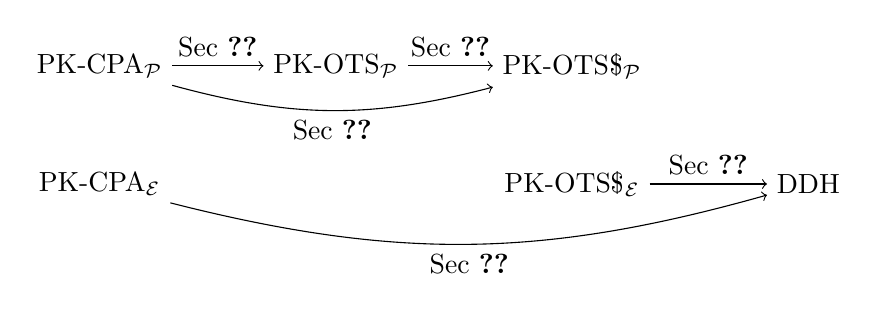
\begin{tikzpicture}
  \node (cpa) at (0,0) {PK-CPA$_{\P}$};
  \node (ots) at (3,0) {PK-OTS$_\P$};
  \node (otsr) at (6,0) {PK-OTS\$$_\P$};
  \draw[->] (cpa) to node [midway,above]{Sec \ref{sec:cpaots}} (ots);
  \draw[->] (ots) to node [midway,above]{Sec \ref{sec:otsotsr}} (otsr);
  \draw[->] (cpa) to [bend right=15] node [midway,below]{Sec \ref{sec:cpaotsr}} (otsr);

  \node (cpae) at (0,-1.5) {PK-CPA$_{\mathcal{E}}$};
  \node (otsre) at (6,-1.5) {PK-OTS\$$_\mathcal{E}$};
  \node (ddh) at (9,-1.5) {DDH};
  \draw[->] (otsre) to node [midway,above]{Sec \ref{sec:otsrddh}} (ddh);
  \draw[->] (cpae) to [bend right=15] node [midway,below]{Sec \ref{sec:cpaddh}} (ddh);
\end{tikzpicture}
\end{center}
\caption{In the figure, each arrow indicates a reduction from one game-pair to another game-pair (corresponding to two security properties, respectively), read as ``distinguishing the game-pair on the left of the arrow is at least as hard as distinguishing the game-pair on the right.''}
\label{fig:plan}
\end{figure}


\subsection{Related Work}\label{sec:related}

Secrecy properties for public-key encryption schemes have been studied extensively and are widely used in the cryptographic literature, for example in~\cite{mihir98}.
The fact that PK-OTS\$ (one-time secrecy) implies PK-CPA (many-time secrecy) is ``textbook-material'' and a SSP-style proof is given in~\cite{joy} (Chap. 15). This makes public-key infrastructures that we present here a perfect case study for \NSSP.

Previous formal developments that claim to prove PK-CPA for a public-key encryption scheme give what is our definition of PK-OTS\$.  This is the case for the developments in CertiCrypt~\cite{gilles09},  EasyCrypt~\cite{barthe11,husling22} and  FCF~\cite{petcher15fcf}. The reduction from PK-OTS\$ to PK-CPA is an implied relationship and to our knowledge has not been mechanically verified using a proof assistant.

EasyCrypt\footnote{\url{https://github.com/EasyCrypt/easycrypt/blob/b3f68885e9f8ebd5cec64e80d58b1b6f1e9b1971/theories/encryption/PKE_hybrid.ec}} defines and gives
a proof that one-time secrecy implies many-time secrecy. We were not able
to identify this theorem as part of a publication or its use anywhere else.
Compared to our proof, the referenced proof is not done in SSP-style,
but rather it is done in the ``experiment'' style, where ``the bit'' is an internal
random choice and the adversary is called by the experiment rather than the
adversary calling into games as is the case for SSP style proofs.

SSProve~\cite{haselwarter23popl}\footnote{\url{https://github.com/SSProve/ssprove/blob/b5b89d660567d676b5c25533dae58dd397414593/theories/Crypt/examples/AsymScheme.v}} gives definitions for PK-OTS\$, PK-OTS and PK-CPA,
but as discovered in~\cite{nssp-preprint} they are wrong in the given form.
The fatal mistake is that key-generation is run inside the encryption oracle (later called QUERY). This
means that the public key is not fixed throughout the game, as it should be. As a consequence the reduction
from PK-OTS\$ to PK-CPA is not possible, since it crucially relies on a fixed public key. The mechanization in \NSSP is correct: We provide robust and re-usable definitions for PK-OTS\$ and PK-CPA as SSP-style
games, mechanize the parametric reduction from PK-OTS\$ to PK-CPA, and then instantiate it for the ElGamal implementation of a PKE scheme to show that DDH implies PK-CPA.

\subsection{Contributions}\label{sec:contrib}

\begin{itemize}
    \item We introduce Nominal-SSProve, a proof assistant for mechanizing state-separating proofs that allows for clear and concise high-level reasoning.
    \item We introduce a methodology for development of modular cryptographic properties and proofs.
    \item We give the first formally verified concrete security reduction from CPA to OTS\$.
    \item We resolve the missing proof left by SSProve~\cite{haselwarter23popl} and fix the mistakes in the definitions regarding CPA and OTS games.
\end{itemize}


\section{Nominal-SSProve} \label{sec:nominalSSProve}

In state-separating proofs~\cite{brzuska18asiacrypt}, a cryptographic security property of a given cryptographic scheme is expressed as a game-pair. In order to prove the security property true, we show that an arbitrarily chosen adversary who interacts with one of the two games, can only guess up to  a certain probability bound which of the two games he is interacting with. Conventionally, the adversary is probabilistic and polynomial-time computable and the bound is a negligible function indexed by a security parameter, for example, the bit length of a key or similar. For this presentation, however, we ignore both requirements and focus instead on the mechanization of the arguments justifying these bounds and how to formulate inductive and parametric game-hopping arguments in \NSSP.

In general, a game-hopping argument goes as follows. Given the assumption that a given scheme is secure, we devise a sequence of games to construct a bound for the attacker to distinguish the game-pair defined by the target  property, using the triangle inequality, existing bounds by computational assumptions, and other mathematical facts.  Adversaries, games, and reductions are expressed in \NSSP in a unified way as modules that can be composed, rewritten, and reduced. 

In \cref{sec:lang} we introduce the language used to express functions and modules.
In \cref{sec:advantage} we introduce module composition and relevant algebraic rules.
In \cref{sec:method} we introduce the methodology for expressing and proving security properties.


\subsection{Language}\label{sec:lang}

A module is a collection of functions that implement the functionality related to the task at hand: a module can implement an adversary, a security game, or a reduction. A module is defined by input and output interfaces,  it has internal state for storing values shared between function calls, for example, public keys, nonces, message history and the like.

\NSSP inherits the probabilistic language from SSProve for writing security games-as-modules.
The language supports state-variables that persist in-between calls to the module. These
state-variables are called locations and represented by \M{l}.
The argument and return types of modules are restricted to a small universe of types called \texttt{choice\_type} represented by \M{T}.
Identifiers from other modules are represented by \M{F}.
The language is a shallow embedding in Coq, so we let \M{x} represent a Coq variable and \M{v} represent a Coq value.
The grammar for code \M{c} captures the different syntactic categories used to express the code. 
 
\bgroup
\setlength\tabcolsep{2pt}
\begin{center}
\begin{tabular}{rl}
  \M{c} ::=&\M{ret v}
  | \M{x <- c ;; c'}
  | \M{x <- get l ;; c}
  | \texttt{\#}\M{put l := v ;; c}
  | \M{x <- sample v ;; c} \\
  |&\M{if v then c else c'}
  | \M{match v with None => c | Some x => c' end}
  | \texttt{\#}\M{assert v ;; c} \\
  |&\M{call F T T' v}
  | \M{getNone l ;; c}
  | \M{x <- getSome l ;; c}
\end{tabular}
\end{center}
\egroup

We explain the semantics of the constructs.
The first two constructs represent monadic return and bind i.e.
\M{ret} encapsulates the value, and bind runs \M{c} and binds
the resulting value to name \M{x} in \M{c'}.
\M{get} reads from location \M{l} and binds the result to \M{x} in \M{c}.
\M{put} writes value \M{v} to location \M{l}.
\M{sample} makes a random choice according to a distribution given as \M{v}.
\M{if} runs code \M{c} when boolean value \M{v} is true and \M{c'} otherwise.
\M{match} runs code \M{c} when value \M{v} is \M{None} and \M{c'} otherwise.
\M{assert} fails if \M{v} is false.

The last line of constructs are  defined exclusively in Nominal-SSProve, greatly simplifying syntax from SSProve.
\M{call} invokes a function from the underlying module.
\M{getNone} reads the location \M{l} and asserts that it is none.
\M{getSome} reads the location \M{l}, asserts that it is a some value and then unwraps it.

Interfaces and modules are given by the following grammar.

\begin{center}
\begin{tabular}{ll}
\M{I} ::= \M{[interface S1 ; S2 ;} \ldots \M{; Sn ]} &
  \M{S} ::= \texttt{\#}\M{val}\ \texttt{\#}\M{[F] T -> T'} \\
\M{M} ::= \M{[module L ; D1 ; D2 ;} \ldots \M{; Dn ]} &
  \M{D} ::= \texttt{\#}\M{def}\ \texttt{\#}\M{[F] (x : T) : T' { c }}
\end{tabular}
\end{center}

Code that returns a value of type \M{T} is considered well-formed with regard to a set of locations \M{L} and an import interface \M{I} written \texttt{code L I T}.
A module aggregates well-formed functions of type \M{T -> code L I T'} into a well-formed  \M{module I E}, which is said
to have imports \M{I} and exports \M{E}.

\subsection{Advantage}\label{sec:advantage}

Adversarial advantage, i.e.\ the probability of the adversary to guess correctly the game with which he is interacting with, is based on interaction, which is expressed formally using module composition.
Modules can be composed sequentially written $M \circ M'$, which corresponds to inlining function calls in the left module by implementations from the right module.
In Nominal-SSProve, state variables are automatically being renamed from one another using nominal sets to avoid state variable capture across modules. In high-level arguments, this renaming is semantically transparent and allows for stronger reasoning principles than in SSProve where disjointness arguments have to be carried out explicitly.
Two modules that are equal up to variable renaming are said to be $\alpha$-equivalent, written as $M \equiv M'$.
Sequential composition is associative up to $\alpha$-equivalence.
$$ (M \circ M') \circ M'' \equiv M \circ (M' \circ M'') $$

Modules also support parallel composition, which refers to the union of the left and right module (sometimes written $M\ ||\ M'$). We do not use parallel composition in this paper, so we do not discuss that type of composition further.

Let $I$ be an interface. An $I$-game is a game with no imports and \emph{exports} $I$. In contrast, and $I$-adversary has \emph{imports} $I$ and exports one function \texttt{RUN : unit -> bool}.
The advantage between two $I$-games $G$ and $G'$ for a specific $I$-adversary
$\A$ is defined to be
$$\Adv_{G,G'}(\A) =
  |\,\mathrm{Pr}[\texttt{true} \leftarrow (\A \circ G).\texttt{RUN}() ]
  - \mathrm{Pr}[\texttt{true} \leftarrow (\A \circ G').\texttt{RUN}()]\,|,$$
where $\mathrm{Pr}[\texttt{true} \leftarrow M.\texttt{RUN}()]$ is the
probability that evaluating function $\texttt{RUN}$ in $M=\A \circ G$ or $M=\A \circ G'$ returns $\texttt{true}$.  Directly from this definition follows the triangle inequality
$$\Adv_{G,G''}(\A) \leq \Adv_{G, G'}(\A) + \Adv_{G', G''}(\A)$$
for $I$-games $G$, $G'$, $G''$, and $I$-adversary $\A$,
which allows us to ``hop'' through an intermediate game.
Furthermore, advantage is symmetric and $\alpha$-equivalent games
 have advantage $0$, i.e.\ 
$$\Adv_{G, G'}(\A) = \Adv_{G', G}(\A)\qquad G \equiv G' \Rightarrow \Adv_{G, G'}(\A) = 0$$
for $I$-games $G$, $G'$ and $I$-adversary $\A$.
From associativity of sequential composition we derive the reduction lemma
$$\Adv_{R \circ G, R \circ G'}(\A) = \Adv_{G, G'}(\A \circ R)$$
for $I$-games $G$, $G'$, an $E$-adversary $\A$ and a reduction expressed as module $R$ with imports $I$ and exports $E$.

$I$-games $G$ and $G'$ that have $\Adv_{G, G'}(\A) = 0$ for all adversaries are said to be \emph{perfectly indistinguishable} written $G \approx_0 G'$.
For this to be a meaningful definition it is essential that the games and
the adversary do not share state-variables, which is automatically provided by nominal sets in \NSSP.

The fact that two modules are perfectly indistinguishable is usually shown
in the probabilistic relation Hoare logic (pRHL). 
Nominal-SSProve only makes small improvements relative to SSProve with regard to the pRHL, so we will not place any emphasis on these results and only state and explain the lemmas concerning perfect indistinguishability.

In \NSSP, for reasoning about advantages, games may be substituted for another as long as they are perfectly indistinguishable. For more details about this fact, see~\cite{nssp-preprint}.

\cref{tab:translation} shows the translation of state-separating proof concepts into the syntax of Nominal-SSProve as used for formulating theorems throughout this paper, and the proofs in the supplementary materials.



\begin{table}
  \begin{center}
  \begin{tabular}{c|c|c}
    \textbf{State-separating proofs} & \textbf{Notation} & \textbf{Nominal-SSProve} \\
    Protocol & $\mathcal{P}$ & \texttt{Record P := \{ ... \}.} \\
    Interface & I, E & \texttt{I E : Interface} \\
    Module & M & \texttt{M : module I E} \\
    I-adversary & $\A$ & \texttt{A : adversary I} \\
    I-game & $G$ & \texttt{G : game I} \\
    I-game-pair & $\mathrm{GG}$ & \texttt{GG : bool -> game I} \\
    left/real game & $\mathrm{GG^0}$ & \texttt{GG true} \\
    right/ideal game & $\mathrm{GG^1}$ & \texttt{GG false} \\
    Advantage & $\Adv_{G, G'}(\A)$ & \texttt{Adv G G' A} \\
    Advantage for a game-pair & $\Adv_{GG}(\A)$ & \texttt{AdvFor GG A} \\
    Perfectly indistinguishable & $G \approx_0 G'$ & \texttt{perfect I G G'} \\
  \end{tabular}
  \end{center}
  \caption{Correspondence between SSP concepts and Nominal-SSProve}
  \label{tab:translation}
\end{table}

\subsection{Methodology}\label{sec:method}

To model statements about cryptographic protocols we propose taking a
parametric approach that we follow in the case study below.

\begin{itemize}
\item \emph{Schemes} are modeled as record types that declare the names of the base types and the types of the cryptographic algorithms that an implementation of such a scheme would have to provide. For example schemes include public-key scheme, commitment scheme, symmetric encryption scheme, $\Sigma$-protocols and so on.

\item \emph{Security properties} are game-pairs that provide implementations of the functions required by a common interface, capturing the relevant and desired security aspects. A security property is always parameterized by a scheme. The security property's formulation does not depend on the implementation of a scheme but only on the scheme itself. Examples of security properties are \OTSR, \CPA, special honest verifier zero-knowledge (for ZK-schemes), hiding (for commitment schemes), and so on.

\item \emph{Implementations} are values of the record type representing a scheme.  Such a value is an $n$-tuple that declares base types, and gives concrete implementations of the required cryptographic algorithms.
  Examples of implementations include ElGamal, Pallier, Schnorr (for ZK-schemes), Pedersen commitment, and so on.

\item \emph{Security bounds} show a limit to the advantage of an adversary to successfully distinguish between the games modeling a security property for a specific implementation.
  For example we show later in this paper that the \CPA\ advantage for ElGamal can be expressed in terms of the advantage for \DDH. Other examples, beyond the scope of this paper, include a proof that the advantage for special honest verifier zero-knowledge for Schnorr is 0, or a proof that the transformation of a $\Sigma$-protocol into a commitment scheme has the hiding property bounded by the advantage for special-honest verifier zero-knowledge of the $\Sigma$-protocol.
\end{itemize}

The diagram in \cref{fig:deps} summarizes the relationship between the different concepts.


\begin{figure}
\begin{center}
  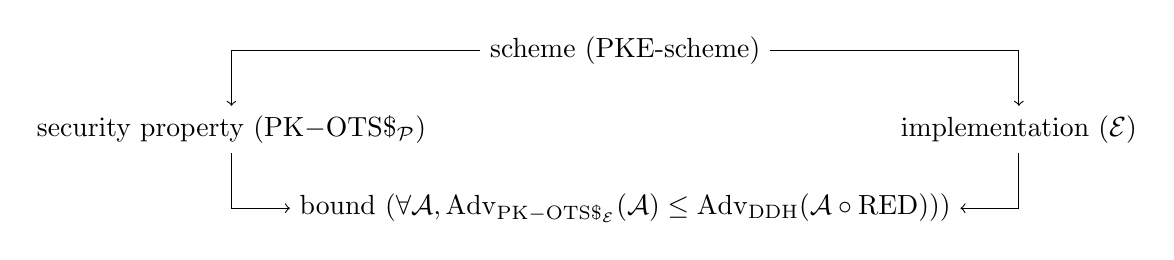
\begin{tikzpicture}
    \node (scheme) at (0,0) {scheme (PKE-scheme)};
    \node (property) at (-5,-1) {security property (\OTSR$_\P$)};
    \node (implementation) at (5,-1) {implementation ($\mathcal{E}$)};
    \node (bound) at (0,-2) {bound ($\forall \A, \Adv_{\OTSR_\mathcal{E}}(\A) \leq \Adv_{\DDH}(\A \circ \RED)) $)};
    \draw[->] (scheme.west) -| node [midway,above]{ } (property.north);
    \draw[->] (scheme.east) -| node [midway,above]{ } (implementation.north);
    \draw[->] (property.south) |- node [midway,below]{ } (bound.west);
    \draw[->] (implementation.south) |- node [midway,below]{ } (bound.east);
  \end{tikzpicture}
  \caption{The diagram shows dependencies between concepts. The parenthesis contains an example.
           An arrow reads as ``is used to define''.}
  \label{fig:deps}
\end{center}
\end{figure}


\section{Public Key Scheme}\label{sec:pkscheme}

We turn now to the case study that we discuss in  this paper.  A public-key encryption (PKE) scheme (also called an asymmetric encryption scheme) is an encryption scheme that uses different keys for encryption and decryption. We illustrate how to carry out abstract security proofs in \NSSP, using quantification over schemes. In our case, we prove that, using abstraction, \emph{any implementation of the PKE scheme} depicted in \cref{fig:pkscheme}, we can reduce chosen plaintext attacks security (\CPA) to one time secrecy random (\OTSR). Then,  we  instantiate this proof to a concrete implementations of the PKE scheme, namely the ElGamal crypto system. 

\begin{figure}
  \begin{minipage}[t]{0.49\textwidth}
    \inputminted{coq}{snippets/pkscheme.v}
    \caption{Defining \texttt{pk\_scheme}}
    \label{fig:pkscheme}
    \inputminted{coq}{snippets/corr.v}
    \caption{Defining correctness games}
    \label{fig:correct}
  \end{minipage} \hfill \begin{minipage}[t]{0.49\textwidth}
    \inputminted{coq}{snippets/init.v}
    \caption{Defining init procedure}
    \label{fig:init}
    \inputminted{coq}{snippets/pkcpa.v}
    \caption{PK-CPA game-pair}
    \label{fig:pkcpa}
  \end{minipage}
\end{figure}


Schemes are modeled in \NSSP as records, where the relevant sets defining a scheme are expressed using \M{choice_type}, and the cryptographic algorithms defined by the scheme are declared by their respective types. 
For PKE schemes,  the relevant sets represent secret keys \M{Sec}, public keys \M{Pub}, messages \M{Mes}, and ciphertexts \M{Cip}. \M{sample_Cip} defines an algorithm for sampling a random ciphertext. \M{keygen} generates and returns
a secret key and a public key that correspond to each other. \M{enc}
encrypts a message using the public key and returns the ciphertext.
\M{dec} decrypts a ciphertext using the secret key and returns the message.

For increased readability, we define syntactic sugar, so that for \M{P : pk_scheme}, the notation \M{'sec P},
\M{'pub P}, \M{'mes P}, \M{'cip P} projects the respective \M{choice_type} from the record \M{P}. Note that schemes declare cryptographic algorithms, they do not implement them. 



\subsection{Correctness}\label{sec:correctness}

Not all implementations of a PKE scheme are correct: At the very minimum, we should expect that the decryption of a ciphertext with the secret key that corresponds to the public key should be the identity. In state separating proofs such a correctness property is captured by the indistinguishability of two games \M{CORR0} and \M{CORR1} depicted in \cref{fig:correct}.
The game \M{CORR0} implements what is commonly referred to as \emph{real} functionality, which makes precise the steps necessary to decrypt an encrypted  message \M{m}. In contrast, the game \M{CORR1} defines the \emph{ideal} functionality, which is, in this case, the identity.  \M{CORR0} is also referred as to as \emph{real game}, whereas \M{CORR1} is called the \emph{ideal game}. 
  
Recall that adversaries are modeled by modules and that adversaries interact with games by module composition, also called linking. In the general case, the game-pair (\M{CORR0}, \M{CORR1}) captures correctness by the following argument: 
If we can prove that an adversary has a low probability of
distinguishing whether it has been linked (to interact with) the real or the ideal game, the
PKE-scheme must have a high probability ($1-\epsilon$) of returning exactly the
original message after encrypting and decrypting it. We say that the PKE-scheme is \emph{$\epsilon$-correct}. In the special case of $\epsilon = 0$, i.e.\ we can prove that that it is impossible for the adversary to distinguish if it has been linked to the real or ideal game, the PKE-scheme is called \emph{perfectly correct}.

The secrecy properties that we elaborate on in \cref{sec:secrecy} do not make use of decryption,
so it is only correctness that makes a formal connection between \M{enc} and \M{dec}, Thus our formalization
would be incomplete without a proof of correctness.
In Section~\ref{sec:elgamal} we provide as an example an implementation of a perfectly correct PKE-scheme and mechanize the correctness proof in \NSSP.
 


\subsection{Secrecy properties - PK-OTS\$, PK-OTS and PK-CPA}\label{sec:secrecy}

As the first secrecy property we introduce one-time secrecy random modeled by games
\OTSR\ defined in \cref{fig:pkotsr}.
In short, \OTSR\ defines a game-pair in the real vs.\ ideal paradigm.
$\OTSR^0$ defines the real functionality by once encrypting a message that is chosen by the adversary.
$\OTSR^1$ defines the ideal functionality by sampling a random ciphertext.
If we can prove that it is infeasible for an adversary to distinguish the games, then the message
is well hidden within the ciphertext.

Each \OTSR\ game defines two functions, namely \M{GET} and \M{QUERY}.
To implement the functions we define an initialization procedure \M{init} in \cref{fig:init},
which is used by all of the secrecy games. \M{init} is responsible for either generating or retrieving
a previously generated public-key, so that it is constant throughout the calls to the game.
\M{GET} returns the public-key to make it available to the adversary before calls to query.
\M{QUERY} uses a flag to check if it has been called before. If it has not, then it either encrypts
the given message or samples a random ciphertext depending on the parameter \M{b} (denoting if it should perform the real or ideal functionality) and returns the result.

The next two game-pairs define secrecy in the left vs.\ right paradigm.
This means that the adversary inputs two
messages and the left game will encrypt and return the left message while the right game will encrypt and return the right message.

We define the left vs.\ right version of one-time secrecy \OTS\ in \cref{fig:pkots}.
\OTS\ defines two functions \M{GET} and \M{QUERY} just like \OTSR, except that \M{QUERY} takes two messages.

The two game-pairs capturing  one-time secrecy (\OTS\ and \OTSR) are related in that the advantage for \OTS\ can be
expressed in terms of the advantage for \OTSR, and so we say that \OTS\ reduces to \OTSR.
Intuitively, the proof is simple: To bound the advantage for \OTS, we hop from
left to random by \OTSR\ and then hop from random to right again by \OTSR.
We do the proof formally in \cref{sec:otsotsr} by defining a reduction module.

Finally, we define a left vs.\ right version of many-time secrecy called \CPA\ in \cref{fig:pkcpa}.
\CPA\ takes a parameter $n$, which determines the maximum number of times that \M{QUERY} may be called.
We are careful to define \CPA\ so that it reuses the public key for each encryption. It would
be a mistake to define \M{QUERY} by calling \M{keygen} to generate a new public key on each call.
In \cref{sec:cpaots} we formally prove, that many-time secrecy \CPA\ reduces to \OTS.
At first glance this is a surprising result, because it is not obvious that we can re-use
the same public key multiple times without revealing some pattern in the outputs. On the other hand,
once the adversary obtains the public key it is free to encrypt as many messages as it wants,
so that process should never reveal anything more about the connection between messages and ciphertexts.
In fact, if we were to develop similar properties for symmetric
encryption (e.g. the one-time pad), this result would not hold. The difference is that there is only a single (secret) key unknown
to the adversary.

In \cref{sec:cpaotsr} we formally combine the reduction from \CPA\ to \OTS\ and
the reduction from \OTS\ to \OTSR\ to make a reduction from \CPA\ to \OTSR.


\begin{figure}
  \begin{minipage}[t]{0.49\textwidth}
    \inputminted{coq}{snippets/pkotsr.v}
    \caption{PK-OTS\$ definition}
    \label{fig:pkotsr}
    \inputminted{coq}{snippets/choose.v}
    \caption{CHOOSE reduction}
    \label{fig:choose}
  \end{minipage} \hfill \begin{minipage}[t]{0.49\textwidth}
    \inputminted{coq}{snippets/pkots.v}
    \caption{PK-OTS definition}
    \label{fig:pkots}
    \inputminted{coq}{snippets/slide.v}
    \caption{SLIDE reduction}
    \label{fig:slide}
  \end{minipage}
\end{figure}


\subsection{PK-OTS reduces to PK-OTS\$} \label{sec:otsotsr}

To reduce from \OTS\ to \OTSR\ we define a reduction \CHOOSE\ as shown in \cref{fig:choose}.
\CHOOSE\ implements \M{GET} by calling the underlying module.
\CHOOSE\ implements \M{QUERY} by choosing either the left or the right value according to its boolean parameter and calls \M{QUERY} of the underlying module.

The \OTS\ games can be expressed in terms of the ``real'' \OTSR\ game
using \CHOOSE\ to choose either the left or right message dependent
on \M{b}.

\begin{minted}{coq}
Lemma PK_OTS_CHOOSE_perfect {P} b
  : perfect (I_PK_OTS P) (PK_OTS P b) (CHOOSE P b ∘ PK_OTSR P true).
\end{minted}

When \CHOOSE\ is composed with the ``ideal'' \OTSR\ it does not
matter which message is chosen, so the parameter \M{b} may be changed.

\begin{minted}{coq}
Lemma CHOOSE_perfect {P} : perfect (I_PK_OTS P)
  (CHOOSE P true ∘ PK_OTSR P false) (CHOOSE P false ∘ PK_OTSR P false).
\end{minted}

These lemmas combine with high level advantage reasoning to show
that \OTS\ reduces to \OTSR.

\begin{minted}{coq}
Theorem Adv_PK_OTS_OTSR {P} (A : adversary (I_PK_OTS P)) :
  AdvFor (PK_OTS P) A
  <= AdvFor (PK_OTSR P) (A ∘ CHOOSE P true)
  +  AdvFor (PK_OTSR P) (A ∘ CHOOSE P false).
\end{minted}
\begin{proof}
  Let a scheme $\P$ and a \OTS-adversary $\A$ be given.
  Define $\mathcal{B}_{b'}^b = \CHOOSE_{\P,b'} \circ \OTSR^b_\P$.
  From \M{PK_OTS_CHOOSE_perfect} followed by the triangle equality we have
  $$\Adv_{\OTS_\P}(\A)
    = \Adv_{\mathcal{B}_0^0, \mathcal{B}_1^0}(\A) \leq \Adv_{\mathcal{B}_0^0, \mathcal{B}_0^1}(\A) + \Adv_{\mathcal{B}_0^1, \mathcal{B}_1^0}(\A).$$
  We consider each addend separately. In the first we have
  $$\Adv_{\mathcal{B}_0^0,\mathcal{B}_0^1}(\A) = \Adv_{\OTSR_\P}(\A \circ \CHOOSE_{\P,0})$$
  by reduction.
  In the second we have
  $$\Adv_{\mathcal{B}_0^1,\mathcal{B}_1^0}(\A) = \Adv_{\mathcal{B}_1^1,\mathcal{B}_1^0}(\A) = \Adv_{\OTSR_\P}(\A \circ \CHOOSE_{\P,1})$$
  by \M{CHOOSE_perfect}, symmetry, and reduction which concludes the proof.
\end{proof}



\subsection{PK-CPA reduces to PK-OTS} \label{sec:cpaots}

To reduce from \CPA\ to \OTS\ we introduce a reduction module called
\SLIDE\ defined in \cref{fig:slide} that lets us
gradually change from encrypting the left
message to encrypting the right message.
\SLIDE\ has three parameters.
The first is the implementation of a scheme $\P$, which lets
\SLIDE\ depend on its types and lets its definition depend on the types
of the implementation.
The second parameter is $i$, controls when to encrypt which message.
\SLIDE\ has an internal counter to count the number of encrypted messages.
When the counter is less than $i$, the right message gets encrypted.
When the counter is exactly $i$, then \SLIDE\ calls the \M{QUERY} function of the underlying module.
When the counter is greater than $i$, the left message gets encrypted.
The third parameter is $n$, which controls the maximum number of messages
that \SLIDE\ will encrypt.
\SLIDE\ also defines the function \M{GET}, which is simply implemented by
calling the underlying module. Likewise, \SLIDE\ relies on the underlying
module to return the public key for encryption.

We prove two lemmas \SLIDE\ in the pRHL.
The first lemma shows that \SLIDE\ behaves just as \CPA$^0$ when $i = 0$
and as \CPA$^1$ when $i = n$.

\begin{minted}{coq}
Lemma PK_CPA_SLIDE_perfect {P n} b : perfect (I_PK_CPA P)
  (PK_CPA P n b) (SLIDE P (if b then 0 else n) n ∘ PK_OTS P true).
\end{minted}

The second lemma shows that when the underlying module encrypts the
right message we might as well increase the parameter to $i+1$.
The proof is completed by considering the different cases for the
relative size of the \SLIDE\ counter and $i$.

\begin{minted}{coq}
Lemma SLIDE_succ_perfect {P} {n} {i} : perfect (I_PK_CPA P)
  (SLIDE P i n ∘ PK_OTS P false) (SLIDE P i.+1 n ∘ PK_OTS P true).
\end{minted}

We combine these lemmas to make $n$ ``hops'' in total
to obtain a reduction from \CPA\ to \OTS.

\begin{minted}{coq}
Theorem Adv_PK_CPA_OTS {P} {n} (A : adversary (I_PK_CPA P)) :
  AdvFor (PK_CPA P n) A <= \sum_(0 <= i < n) AdvFor (PK_OTS P) (A ∘ SLIDE P i n).
\end{minted}
\begin{proof}
  Let a scheme $\P$, $n \in N$ and a \CPA-adversary $\A$ be given.
  Define $\mathcal{B}_i^b = \SLIDE_{\P, i, n} \circ \OTS_\P^b$.
  Then
  $$\Adv_{\CPA_{\P,n}}(\A)
    = \Adv_{\SLIDE_{\P, 0, n} \circ \OTS_{\P}^0,
            \SLIDE_{\P, n, n} \circ \OTS_{\P}^0 }(\A) = \Adv_{\mathcal{B}_0^0,\mathcal{B}_n^0}(\A)$$
  by \M{PK_CPA_SLIDE_perfect}.
  We proceed by induction on $n$.
  \begin{itemize}
  \item In the base case, from the fact that the sum is empty we have
  $$\Adv_{\mathcal{B}_0^0, \mathcal{B}_0^0}(\A)
      = 0 = \sum_{0 \leq i < 0} \Adv_{\OTS_\P}(\A \circ \SLIDE_{\P,i,n}).$$
  \item In the inductive case assume that 
    $$\Adv_{\mathcal{B}_0^0, \mathcal{B}_j^0}(\A) \leq
      \sum_{0 \leq i < j} \Adv_{\OTS_\P}(\A \circ \SLIDE_{\P,i,n}).$$
    Observe that by \M{SLIDE_succ_perfect} and reduction
      $$\Adv_{\mathcal{B}_j^0,\mathcal{B}_{j+1}^0}(\A)
      = \Adv_{\mathcal{B}_j^0,\mathcal{B}_{j}^1}(\A) 
      = \Adv_{\OTS_\P}(\A \circ \SLIDE_{\P,j,n}).
      $$
    We combine this with the induction hypothesis and get
    $$
        \Adv_{\mathcal{B}_0^0, \mathcal{B}_{j+1}^0}(\A) \leq
        \Adv_{\mathcal{B}_0^0, \mathcal{B}_j^0}(\A)
        + \Adv_{\mathcal{B}_j^0, \mathcal{B}_{j+1}^0}(\A) \\
        \leq \sum_{0 \leq i < j+1} \Adv_{\OTS_\P}(\A \circ \SLIDE_{\P,i,n}),
        $$
    which finishes the proof.
  \end{itemize}
\end{proof}

\subsection{PK-CPA reduces to PK-OTS\$} \label{sec:cpaotsr}

We combine the \OTS\ to \OTSR\ reduction with the \CPA\ to \OTS\ reduction
to derive a \CPA\ to \OTSR\ reduction.

\begin{minted}{coq}
Theorem Adv_PK_CPA_OTSR {P} {n} (A : adversary (I_PK_CPA P)) :
  AdvFor (PK_CPA P n) A <= \sum_(0 <= i < n)
    ( AdvFor (PK_OTSR P) (A ∘ SLIDE P i n ∘ CHOOSE P true)
    + AdvFor (PK_OTSR P) (A ∘ SLIDE P i n ∘ CHOOSE P false) ).
\end{minted}
\begin{proof}
  Let a scheme $\P$, $n \in \mathbb{N}$ and a \CPA-adversary $\A$ be given.
  Define $\mathcal{B}_i = \mathcal{A} \circ \SLIDE_{\P,i,n}$. Then
  \begin{align*}
    \Adv_{\CPA_{\P,n}}
    \leq \sum_{0 \leq i < n}\ &\Adv_{\OTS_{\P}}(\mathcal{B}_i) \\
    \leq \sum_{0 \leq i < n}\ &\Adv_{\OTSR_{\P}}(\mathcal{B}_i \circ \CHOOSE_{\P,0}) \\
    +\ &\Adv_{\OTSR_{\P}}(\mathcal{B}_i \circ \CHOOSE_{\P,1}).
  \end{align*}
  by \M{Adv_PK_CPA_OTS} followed by \M{Adv_PK_OTS_OTSR} on each addend.
\end{proof}

The previous theorem gives us an exact bound where the only difference
in the different addends of the sum is in the construction of the adversary.
It may be permissible to relax the bound by choosing some \M{p}
that is proven to be a common bound for each of the adversaries.
This intent is captured by the following corollary.

\begin{minted}{coq}
Corollary Adv_CPA_OTSR_p {P} {n} {p} (A : adversary (I_PK_CPA P)) :
  (∀ i b, AdvFor (PK_OTSR P) (A ∘ SLIDE P i n ∘ CHOOSE P b) <= p) →
  AdvFor (PK_CPA P n) A <= p *+ 2 *+ n.
\end{minted}
\begin{proof}
  Let a scheme $\P$, $n \in \mathbb{N}$, $p \in \mathbb{R}$
  and a \CPA-adversary $\A$ be given.
  Define $\mathcal{B}_{i,b} = \A \circ \SLIDE_{\P,i,n} \circ \CHOOSE_{\P,b}$.
  Then

  $$\Adv_{\CPA_{\P,n}}(\A) \leq
    \sum_{0 \leq i < n} \Adv_{\OTSR_\P}(\mathcal{B}_{i,b}) + \Adv_{\OTSR_\P}(\mathcal{B}_{i,b}) \leq
    \sum_{0 \leq i < n} p + p = 2np,$$

  where the first step follows by \M{Adv_PK_CPA_OTSR}, the second step
  follows by the assumption, and the third step is trivial.
\end{proof}

\section{The ElGamal Public Key Scheme}\label{sec:elgamal}

We introduce an implementation of the ElGamal cryptosystem as a public key scheme seen in \cref{fig:elgamal}.
The implementation assumes the existence of a cyclic group $\mathcal{G}$
that has \M{g} as a generator.
\M{'fin}\ \texttt{\#}\M{|el|} and \M{'fin}\ \texttt{\#}\M{|exp|} represents the elements and exponents of $\mathcal{G}$ respectively.
The operators \M{*}, \M{^+}, \M{^-} represent group multiplication, exponentiation and inverse exponentiation respectively.
The fact that Nominal-SSProve is a shallow embedding allows us to inherit
the group structures and theorems of mathcomp~\cite{mathcomp-group}
now based in Hierarchy Builder~\cite{hb}.

\subsection{ElGamal is perfectly correct}\label{sec:elgamalcorrect}

To begin with, we prove that ElGamal is perfectly correct,
i.e.\ for all adversaries (even the computationally unconstrained)
the two correctness games \M{CORR0} and \M{CORR1} are perfectly indistinguishable. We prove this in the pRHL and in essence is about solving the usual group
equations to prove correctness for ElGamal.
\begin{minted}{coq}
Theorem correct_elgamal : perfect (I_CORR elgamal) (CORR0 elgamal) (CORR1 elgamal).
\end{minted}

\subsection{PK-OTS\$ for ElGamal reduces to DDH} \label{sec:otsrddh}

We now prove that \OTSR\ for ElGamal reduces to \DDH.
This means that we can find a reduction such that for any adversary,
the chance that the adversary distinguishes between \OTSR\ games is the same as the
adversary distinguishing between the \DDH\ games through the reduction. Therefore by contra-position: If we believe
that the DDH assumption is strong enough for the group in question, we must believe in the \OTSR\ security for ElGamal.

\begin{figure}
  \begin{minipage}[t]{0.49\textwidth}
    \inputminted{coq}{snippets/red.v}
    \caption{Reduction from OTS\$ to DDH for ElGamal}
    \label{fig:red}
  \end{minipage} \hfill \begin{minipage}[t]{0.49\textwidth}
    \inputminted{coq}{snippets/elgamal.v}
    \caption{ElGamal definition}
    \label{fig:elgamal}

    \inputminted{coq}{snippets/ddh.v}
    \caption{DDH Definition}
    \label{fig:ddh}
  \end{minipage}
\end{figure}

We define the \DDH\ games in \cref{fig:ddh}
and the reduction module \RED\ in \cref{fig:red}.
First we prove that each \OTSR\ game can be represented as the reduction module composed with their according \DDH\ game.

\begin{minted}{coq}
Lemma PK_OTSR_RED_DDH_perfect b :
  perfect (I_PK_OTSR elgamal) (PK_OTSR elgamal b) (RED ∘ DDH b).
\end{minted}

Then we obtain the desired reduction using high level advantage reasoning.

\begin{minted}{coq}
Lemma OTSR_elgamal (A : adversary (I_PK_OTSR elgamal)) :
  AdvFor (PK_OTSR elgamal) A = AdvFor DDH (A ∘ RED).
\end{minted}
\begin{proof}
  Let a \OTSR-adversary $\A$ be given, then
  $$\Adv_{\OTSR_\mathcal{E}}(\A)
  = \Adv_{\RED \circ \DDH^0, \RED \circ \DDH^1}(\A)
  = \Adv_{\DDH}(\A \circ \RED),$$
  where the first step follows by \M{PK_OTSR_RED_DDH_perfect} and the second
  step follows by reduction.
\end{proof}

This is the usual security result presented for ElGamal such as in~\cite{gilles09,barthe11,petcher15fcf,haselwarter23popl}.
We shall now see that in our formulation, it can be iterated.
 
  \subsection{PK-CPA for ElGamal reduces to DDH}\label{sec:cpaddh}
 
  To show the application of our main theorem we formally prove, that PK-CPA reduces to DDH for ElGamal.
  We prove the theorem by combining the PK-CPA to PK-OTS\$ reduction and the ElGamal-specific PK-OTS\$ to DDH reduction.
  
  
\begin{minted}{coq}
Theorem CPA_elgamal {n} {p} (A : adversary (I_PK_CPA elgamal)) :
  (∀ i b, AdvFor DDH (A ∘ SLIDE elgamal i n ∘ CHOOSE elgamal b ∘ RED) <= p) →
  AdvFor (PK_CPA elgamal n) A <= p *+ 2 *+ n.
\end{minted}
\begin{proof}
  Let $n \in \mathbb{N}$, $p \in \mathbb{R}$ and a \CPA-adversary be given.
  Define $\mathcal{B}_{i,b} = \A \circ \SLIDE_{\mathcal{E},i,n} \circ \CHOOSE_{\mathcal{E},b}$.
  Note that for all $i \in \mathbb{N}$ and $b \in \{0, 1\}$,
  $$
  \Adv_{\OTSR_{\mathcal{E}}}(\mathcal{B}_{i,b}) =
  \Adv_{\DDH}(\mathcal{B}_{i,b} \circ \RED) \leq p
  $$
  by \M{OTSR_elgamal} and the assumption. Then use the corollary
  \M{Adv_CPA_OTSR_p} 
  to conclude that $\Adv_{\CPA_{\mathcal{E},n}}(\A) \leq 2pn$.
\end{proof}

  This arguement combines several reductions to provide a concrete security bound for the CPA security of ElGamal.
  If we had attempted this argument in either SSProve~\cite{haselwarter23popl}
  or as an SSP-style proof in EasyCrypt~\cite{dupressoir22csf}
  we would have accumulated various disjointness requirements from the reduction modules
  with regard to the adversary.
  In contrast, in Nominal-SSProve theorems are free of such side-conditions since disjointness
  is automatic.
  

\section{Conclusion}\label{sec:conclusion}

We introduce Nominal-SSProve and show how it can be used to develop abstract modular
security proofs, that allow long reduction chains as evidenced by the case study.
We also introduce a methodology, that we follow in our case study
where we formalize the reduction from \CPA\ to \OTSR\ for an abstract PKE-scheme,
thereby filling a formalization gap left by previous developments and fixing certain definitions.
We combine the general theory to prove a reduction from \CPA\ to \DDH\ for ElGamal.

\bibliography{../library/library.bib}

%\printbibliography

\end{document}
